\documentclass[paper=letter, fontsize=11pt]{scrartcl}
\usepackage{graphicx}
\usepackage{subcaption}
\usepackage[T1]{fontenc}
\usepackage{fourier}
\usepackage[english]{babel}
\usepackage{amsmath,amsfonts,amsthm}
\usepackage{acronym}
\usepackage{comment}
\usepackage{listings}
\usepackage{framed}
\usepackage{geometry}
\geometry{margin=1in}
\usepackage{sectsty}
\allsectionsfont{\centering \normalfont\scshape}
\usepackage{fancyhdr}
\pagestyle{fancyplain}
\fancyhead{}
\fancyfoot[L]{}
\fancyfoot[C]{}
\fancyfoot[R]{\thepage}
\renewcommand{\headrulewidth}{0pt}
\renewcommand{\footrulewidth}{0pt}
\setlength{\headheight}{13.6pt}
\numberwithin{equation}{section}
\numberwithin{figure}{section}
\numberwithin{table}{section}
\setlength\parindent{0pt}
\newcommand{\horrule}[1]{\rule{\linewidth}{#1}} 
\newcommand{\RNum}[1]{\uppercase\expandafter{\romannumeral #1\relax}}

\title{	
\normalfont \normalsize 
\textsc{University of Victoria, Computer Science Department} \\ [25pt]
\horrule{0.5pt} \\[0.4cm]
\huge CSC-586A Self-Adaptive Systems -- Assignment 2 Part II \\
\horrule{2pt} \\[0.5cm]
}
\author{Ernest Aaron, Simar Arora, Harshit Jain, Stephan Heinemann}
\date{\normalsize\today}

\begin{document}
\maketitle

\clearpage
\section{Part IIa -- \acs{PID} Controller Design}
\label{sec:part2}

\subsection{Resource Control Problem}
\label{sec:resource_control_problem}
\par
Our resource problem can be identified as a queueing model which revolves around
a server. The resource to be managed is the number of tasks to be admitted to
a server which features a certain service time per task. The server may process
tasks in parallel depending on its configuration. If the inter-arrival time of
tasks becomes too short, the load on the server increases and vice versa.
A configurable \ac{FIFO} queue (e.g. queue size) stores tasks that have to wait
for processing while the server is busy. The goal is to keep the number of
waiting tasks at a particular theshold.
\newline
\par
The example is shown in Figure \ref{fig:simulink-server} below and demonstrates
how the queue size for a server is kept in limits by a \ac{PID} controller
that regulates the release of tasks to be completed by the server. Simulink
provides all building blocks of the system that can be configured as desired
(e.g., queue size, concurrency level, service time).
\newline
\par
The first plot shows how the governed inter-arrival time of tasks to be
processed stabilizes. The second plot shows how the number of tasks in the
queue, which shall be kept a level of $10$, stabilizes as well.

\begin{figure}[h]
	\centering
	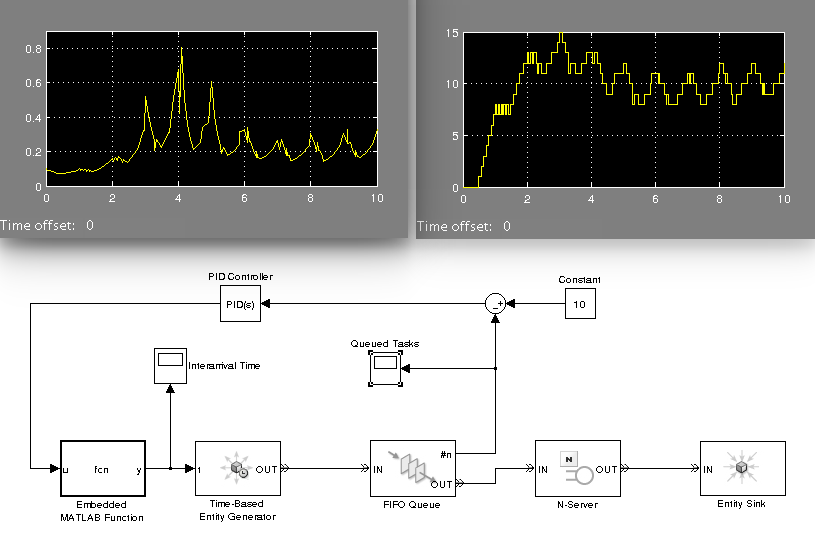
\includegraphics[height=260px]{graphics/simulink-server}
	\caption{Simulink Server Load}
	\label{fig:simulink-server}
\end{figure}

\par
The following tutorial illustrates how to model such resource control systems
using \ac{MATLAB} and its Simulink component as an extension. We decided to
use this extension for our more complex model.

\clearpage
\section{Part IIb -- \acs{PID} Tutorial}
\subsection{System Identification}
\label{sec:system_identification}
\par
The first step to tune (design) a \ac{PID} controller in \ac{MATLAB}, would be
to identify the system to be controlled. In system identification, you need to
find the properties including governing equations, inputs and outputs of your
system. From these characteristics you can create mathematical models that
represent your system (plant). Take for example cruise control: The basic
purpose is to maintain the velocity of a car at a constant.
\newline
\par
The car may experience various disturbances such changes in slope, air drag and
possibly rolling resistance. The introduction of these disturbances can cause
the car to speed up or slow down when going uphill. We see that we need to
employ a mechanism that measures the desired versus the actual velocity and
generates a feedback which aids in keeping the velocity error minimal
regardless of disturbances. Figure \ref{fig:cruise_control_schematic} depicts
a very simplified model of how the velocity of a car changes
\footnote{http://ctms.engin.umich.edu/CTMS/index.php?example=CruiseControl\&section=SystemModeling}.
This model only considers acceleration by the driver and deceleration due to friction
which increases with increasing velocity.

% Astr\"{o}m and Murray\cite{Astrom:2008:FSI:1816978}.

\begin{figure}[h]
	\centering
	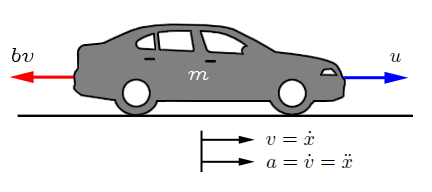
\includegraphics[height=100px]{graphics/cruise-control-schematic}
	\caption{Cruise Control Schematic}
	\label{fig:cruise_control_schematic}
\end{figure}

\par
We can model the change in velocity by the acting forces on the car.
The force required for acceleration is $F_{a} = m * a = m * \ddot{x}$
where $m$ represents the vehicle mass and $a$ its acceleration,
respectively. The force that causes the car to decelerate is
$F_{d} = v * b = \dot{x} * b$ where $v$ represents the current velocity
and $b$ a friction constant that causes a deceleration. The input $u(t)$
to the system is, hence, the sum of the acting forces where the output $y(t)$
is the resulting velocity.

\begin{center}
\begin{framed}
$u(t) = m\ddot{x} + b\dot{x}$, $y(t) = \dot{x}$
\end{framed} 
\end{center}

\subsection{Laplace Transformation and Transfer Function}
\label{sec:laplace_transformation_transfer_function}
\par
Once the system has been identified and the plant has been described by the
governing equations, its transfer function needs to be established. The transfer
function of a system is defined as the relation between its output and input
state

\begin{framed}
\begin{center}
$P(s) = Y(s) / U(s)$
\end{center}
\end{framed} 

where $P(s)$ is the plant transfer function, $Y(s)$ is the output state and
$U(s)$ the input state of the plant. Most (cyber-) physical system equations
depend on time and system behavior is usually described with respect to time.
Hence, the equations usually describe states and their derivatives with respect
to time such as position, speed and acceleration in the cruise control example.

\par
In order to establish the transfer function of a plant, its governing equations
need to be transformed into the frequency (s) domain. The Laplace transform
of a function $f(t)$ is defined as the improper integral.

\begin{framed}
\begin{center}
$\mathcal{L}\{f(t)\} = \int_{0}^{\infty} e^{-st} dt$
\end{center}
\end{framed}

\par
One of the most important rules for differential equations is the Laplace
transform of derivatives that are often found in plant equations

\begin{framed}
\begin{center}
$\mathcal{L}\{f'(t)\} = s \mathcal{L}\{f(t)\} - f(0)$
\end{center}
\end{framed}

where $f(0)$ represents the initial condition with respect to $f$ at time $0$.

\par
Applying the Laplace transform and the above rule to the cruise control example
yields

\begin{framed}
\begin{center}
$P(s) = Y(s) / U(s) = \mathcal{L}\{\dot{x}\} / \mathcal{L}\{\ m\ddot{x} + b\dot{x}\}
= \mathcal{L}\{\dot{x}\} / ms\mathcal{L}\{\dot{x}\} + b\mathcal{L}\{\dot{x}\}
= 1 / (ms + b)$
\end{center}
\end{framed}

\par
The resulting transfer function of the plant (e.g., $1 / (ms + b)$ in the
cruise control example) can then multiplied to other transfer functions in the
control loop in order the reduce the entire system to a single transfer function
as desribed in Section \ref{sec:matlab}. Instead of solving the Laplace
transformation by hand, we could also reference the applicable Laplace tables.

\subsection{\acl{MATLAB}}
\label{sec:matlab}
\par
After identifying your system and deriving your plant transfer function you
can now move on to assembling and simulating your system in \ac{MATLAB}.

\subsection{Cruise Control Parameters}
\label{sec:parameters_cruise_control}
\par
Firstly, you need to define the constants for your modeled plant -- in this
case the cruise control system. The parameters are as follows:

\begin{center}
\begin{framed}
Vehicle Mass $m = 1000 kg$\\
Damping Coefficient $b = 50 Ns/m$\\
Reference Speed $r = 10 m/s$\\
\end{framed}
\end{center}

\subsection{\ac{MATLAB} Implementation}
\label{sec:parameters_cruise_control}
\par
Using the following sequence of commands, you establish a feedback control loop
with the car modeled above being the controlled plant.

\begin{framed}
{\texttt
s=tf('s');         \% define the basic transfer function s\\
m=1000;            \% define the vehicle mass to be 1000kg\\
b=50;              \% define the damping coefficient to be 50Ns/m\\
r=10;              \% define the reference speed to be 10m/s\\
G=1/(m*s + b);     \% define the plant (car) transfer function \\
Kp=1;              \% define the proportional gain\\
Ki=0;              \% define the integral gain\\
Kd=0;              \% define the derivative gain\\
C=pid(Kp,Ki,Kd);   \% construct the PID controller using the gains\\
T=feedback(C*G,1); \% construct the feedback loop with controller and plant\\
t = 0:0.1:20;      \% define the time interval for simulation\\
step(r*T,t)        \% plot the step response of the system in the time interval
}
\end{framed}

\par
The above sequence employs the built-in \ac{PID} controller object which
already abstracts the \ac{PID} transfer function $C = K_{p} + K_{i} / s + K_{d}s$
which you could also define manually. The sequence furthermore uses the feedback
object multiplying all transfer functions in the control loop, that is, $C * G$.
Recall that our transfer function for the car is $G = 1 / (ms + b)$ as derived in section
\ref{sec:laplace_transformation_transfer_function}.
\newline
\par
In general you may want to start your simulation by adjusting the proportional
gain only and then proceed with the remaining gains.
Now you can adjust the values of $Kp$, $Ki$ and $Kd$ to achieve an acceptable
system response. If $Kp = 100$ and $r =10$ (reference speed), the step
response is as shown in Figure \ref{fig:step_kp100}.

\begin{figure}[h]
	\begin{subfigure}{.5\textwidth}
		\centering
	    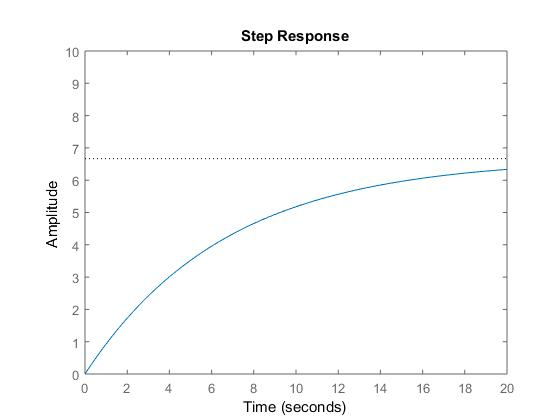
\includegraphics[height=160px]{graphics/step-kp100}\\
		Not acceptable for cruise control.
		The rise time ($14.6$ seconds) is too high and not acceptable.
		The steady state error ($10-6.67 = 3.33$) is too high and not acceptable.
		\caption{Cruise Control Step Response - $K_{p} = 100$}
		\label{fig:step_kp100}
	\end{subfigure}
	\begin{subfigure}{.5\textwidth}
		\centering
	    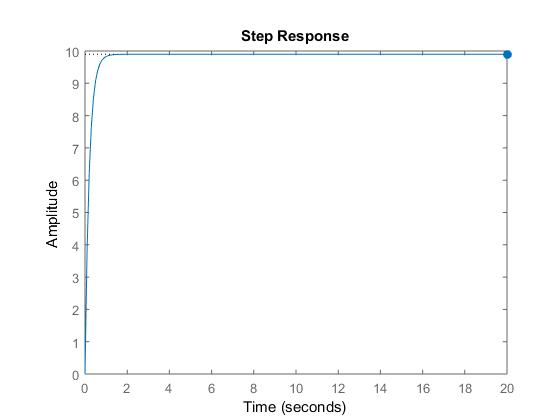
\includegraphics[height=160px]{graphics/step-kp4900}\\
		Not acceptable for cruise control.
		The rise time ($0.445$ seconds) is too short and not acceptable.
		The steady state error is now approximately zero and acceptable.
		\caption{Cruise Control Step Response - $K_{p} = 4900$}
		\label{fig:step_kp4900}
	\end{subfigure}
	\caption{Cruise Control Step Responses I}
	\label{fig:cc_step_responses_i}
\end{figure}

\begin{comment}
\begin{figure}[h]
	\begin{center}
			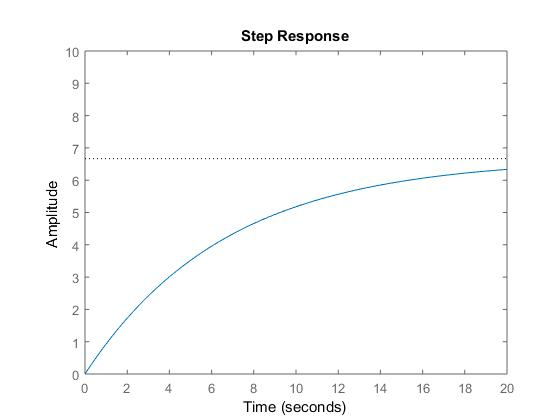
\includegraphics[height=200px]{graphics/step-kp100}\\
			Not acceptable according to our system.
			The rise time ($14.6$ seconds)
			The steady-state error ($10-6.67 = 3.33$)
	\end{center}
	\caption{Cruise Control Step Response - $K_{p} = 100$}
	\label{fig:step_kp100}
\end{figure}
\end{comment}

\begin{comment}
\begin{figure}[h]
	\centering
	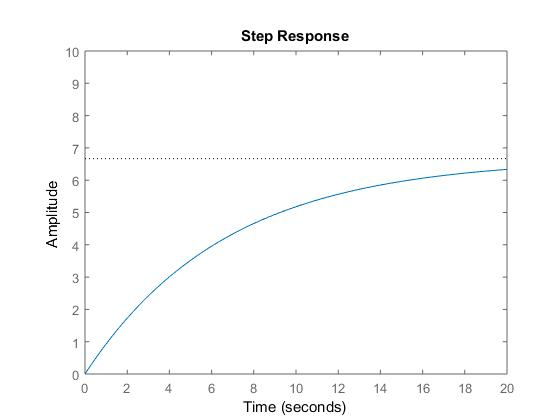
\includegraphics[height=100px]{graphics/step-kp100}
	\caption{Cruise Control Step Response - $K_{p} = 100$}
	\label{fig:step_kp100}
\end{figure}
\end{comment}

\par
The important properties of
the step response are {\em rise time}, {\em overshoot} and {\em settling time}.
You can get these properties from the generated plot by right-clicking on the
graph and selecting the {\em Characteristics} context menu item.
\newline
\par
So we have to increase the value of $Kp$ (proportional gain) because it reduces
the steady state error as well as the rise time but up to a certain limit.
Higher values of $Kp$ lead to overshoot which is not acceptable for the cruise
control system because it leads to oscillations. Short rise times are also
limited by the acceleration performance of the car.
\newline
\par
If $Kp = 4900$ and $r =10$ (reference speed), the step response is as shown in
Figure \ref{fig:step_kp4900}.
Now the system features a very short rise time of about $0.445$ seconds which is
not practically acceptable for the system because the car is unlikely to
accelerate from $0$ to $10 m/s$ in just $0.445$ seconds.
\newline
\par
So we have to add the integral term in the controller and reduce the value
of the proportional gain so its gives the acceptable rise time and the integral
term will eliminate the steady state error. When $Kp = 600$, $Ki=2$ and
$r=10$ (reference speed), the step response is as shown in Figure
\ref{fig:step_kp600_ki2}.

\begin{figure}[h]
	\begin{subfigure}{.5\textwidth}
		\centering
	    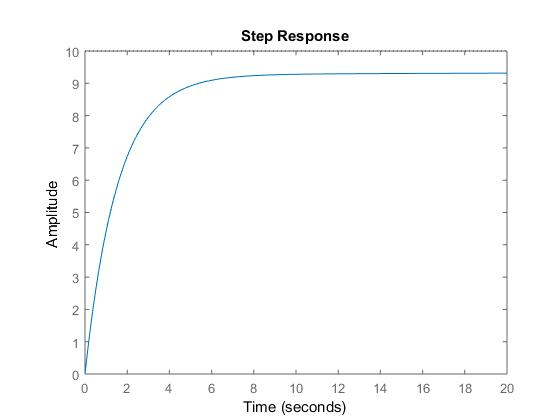
\includegraphics[height=160px]{graphics/step-kp600-ki2}\\
		Less acceptable for cruise control.
		The settling time is very high and not acceptable.
		The steady state error is now zero and acceptable.
		\caption{Cruise Control Step Response - $K_{p} = 600, K_{i} = 2$}
		\label{fig:step_kp600_ki2}
	\end{subfigure}
	\begin{subfigure}{.5\textwidth}
		\centering
	    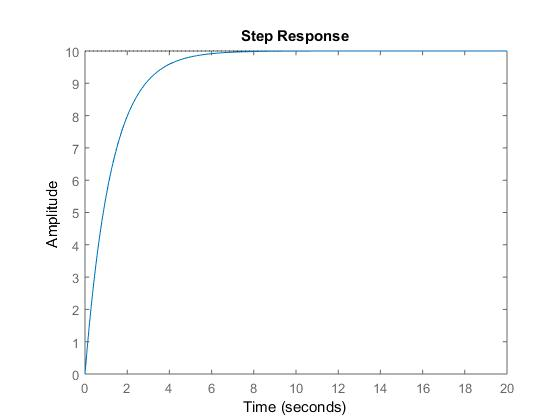
\includegraphics[height=160px]{graphics/step-kp800-ki10}\\
		Acceptable for cruise control.
		The settling time ($4.89$ seconds) is acceptable.
		The rise time ($2.75$ seconds) is acceptable.
		The steady state error is now zero and acceptable.
		\caption{Cruise Control Step Response - $K_{p} = 800, K_{i} = 10$}
		\label{fig:step_kp800_ki10}
	\end{subfigure}
	\caption{Cruise Control Step Responses II}
	\label{fig:cc_step_responses_ii}
\end{figure}

\begin{comment}
\begin{figure}[h]
	\begin{center}
			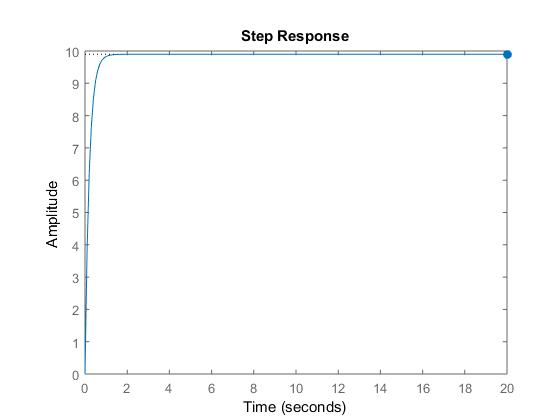
\includegraphics[height=200px]{graphics/step-kp4900}\\
			Not acceptable according to our system.
			The rise time ($0.445$ seconds)
			The Steady state error is now approximately zero.
	\end{center}
	\caption{Cruise Control Step Response - $K_{p} = 4900$}
	\label{fig:step_kp4900}
\end{figure}
\end{comment}

\begin{comment}
\begin{figure}[h]
	\centering
	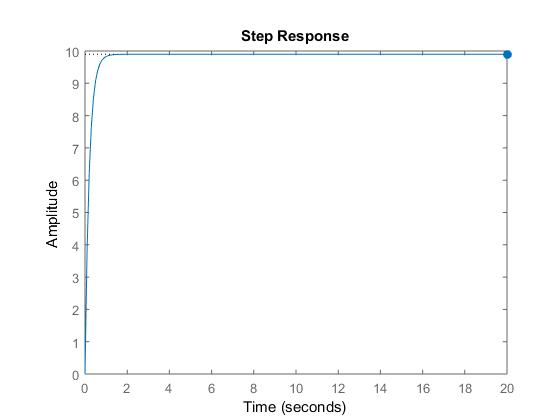
\includegraphics[height=100px]{graphics/step-kp4900}
	\caption{Cruise Control Step Response - $K_{p} = 4900$}
	\label{fig:step_kp4900}
\end{figure}
\end{comment}

\begin{comment}
\begin{figure}[h]
	\begin{center}
			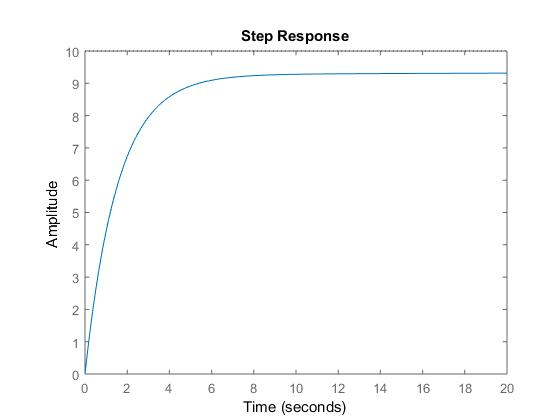
\includegraphics[height=200px]{graphics/step-kp600-ki2}\\
			Less acceptable according to our system.
			The settling time is very high.
			The Steady state error is now zero.
	\end{center}
	\caption{Cruise Control Step Response - $K_{p} = 600, K_{i} = 2$}
	\label{fig:step_kp600_ki2}
\end{figure}
\end{comment}

\begin{comment}
\begin{figure}[h]
	\centering
	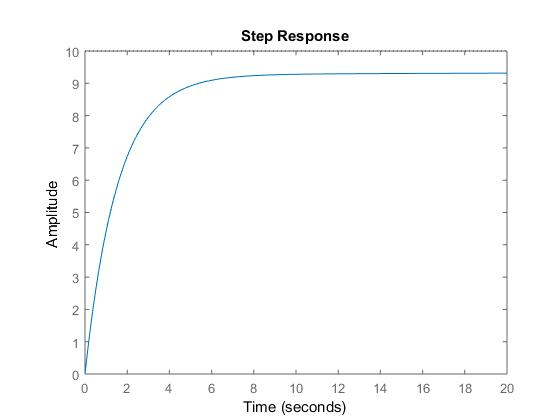
\includegraphics[height=100px]{graphics/step-kp600-ki2}
	\caption{Cruise Control Step Response - $K_{p} = 600, K_{i} = 2$}
	\label{fig:step_kp600_ki2}
\end{figure}
\end{comment}

\par
Now the system is a little more acceptable but the settling time is still
very high.
So we have to adjust both gains (proportional and integral) in such a way
that they result in the desired response. We have to start with a lower value of
$Ki$ because a higher value will destabilize the system. If $Kp = 800$,
$Ki=10$ and $r=10$ (reference speed), the step response is as shown in Figure
\ref{fig:step_kp800_ki10}.

\begin{comment}
\begin{figure}[h]
	\begin{center}
			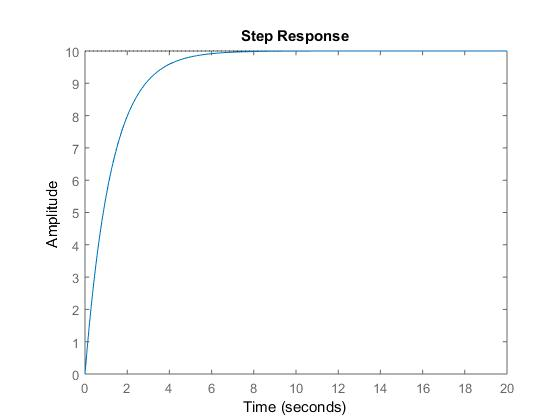
\includegraphics[height=200px]{graphics/step-kp800-ki10}\\
			Acceptable according to our system.
			The settling time ($4.89$ seconds).
			The Rise time ($2.75$ seconds).
			The Steady state error is now zero.
	\end{center}
	\caption{Cruise Control Step Response - $K_{p} = 800, K_{i} = 10$}
	\label{fig:step_kp800_ki10}
\end{figure}
\end{comment}

\begin{comment}
\begin{figure}[h]
	\centering
	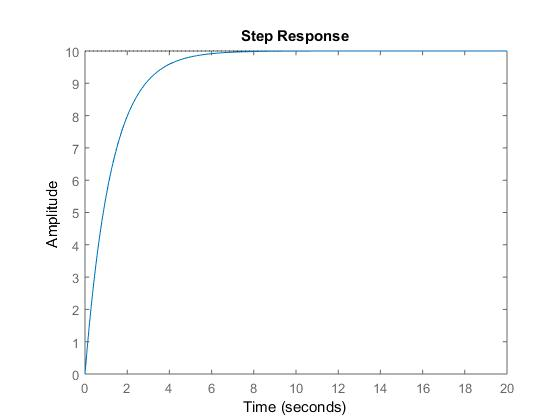
\includegraphics[height=100px]{graphics/step-kp800-ki10}
	\caption{Cruise Control Step Response - $K_{p} = 800, K_{i} = 10$}
	\label{fig:step_kp800_ki10}
\end{figure}
\end{comment}

\par
Now the system is acceptable possessing a suitable settling time, rise
time and zero steady state error. We do not need to add the derivative term
to the controller because we are satisfied with the PI controller.

\subsection{Simulink}
\label{sec:simulink}
\par
More often than not we may need to model systems that are highly complex or in
hindsight the equation is not known. Simulink provides a graphical programming
environment that allows us to use components that already have the transfer
function built into them. Simulink can be accessed through \ac{MATLAB} by typing
the command {\texttt simulink}. If you are given the following \ac{LTI} system
as in Figure \ref{fig:lti_system}, without knowing the \ac{MATLAB} command line
statements, as demonstrated in Section \ref{sec:matlab}, you could open Simulink
and replicate the following system.

\begin{figure}[h]
	\begin{subfigure}{.4\textwidth}
		\centering
	    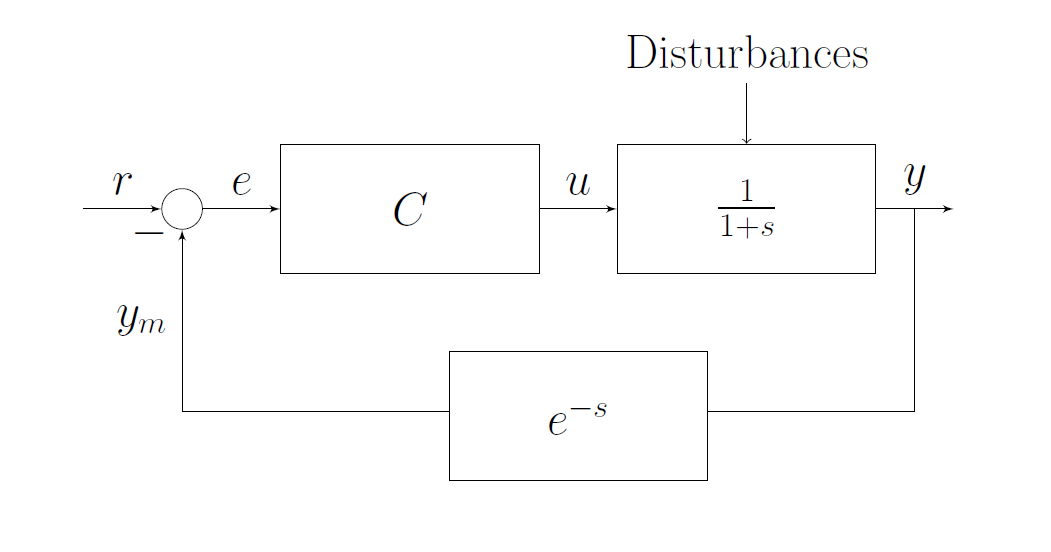
\includegraphics[width=200px]{graphics/lti-system}
		\caption{\acs{LTI} System}
		\label{fig:lti_system}
	\end{subfigure}
	\begin{subfigure}{.6\textwidth}
		\centering
	    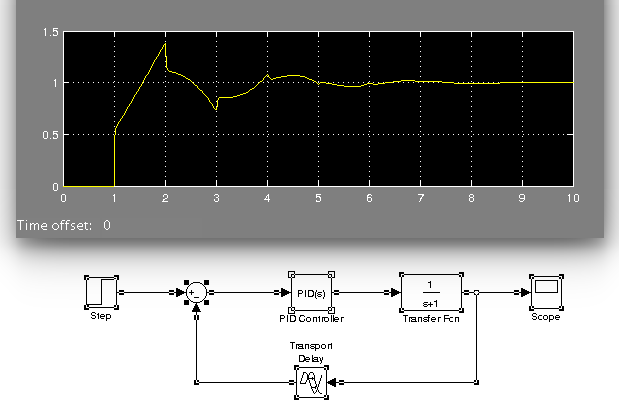
\includegraphics[width=260px]{graphics/simulink-lti}
		\caption{Simulink \acs{LTI} System}
		\label{fig:simulink_lti}
	\end{subfigure}
	\caption{\ac{LTI} System Model}
	\label{fig:lti_system_model}
\end{figure}

\begin{comment}
\begin{figure}[h]
	\centering
	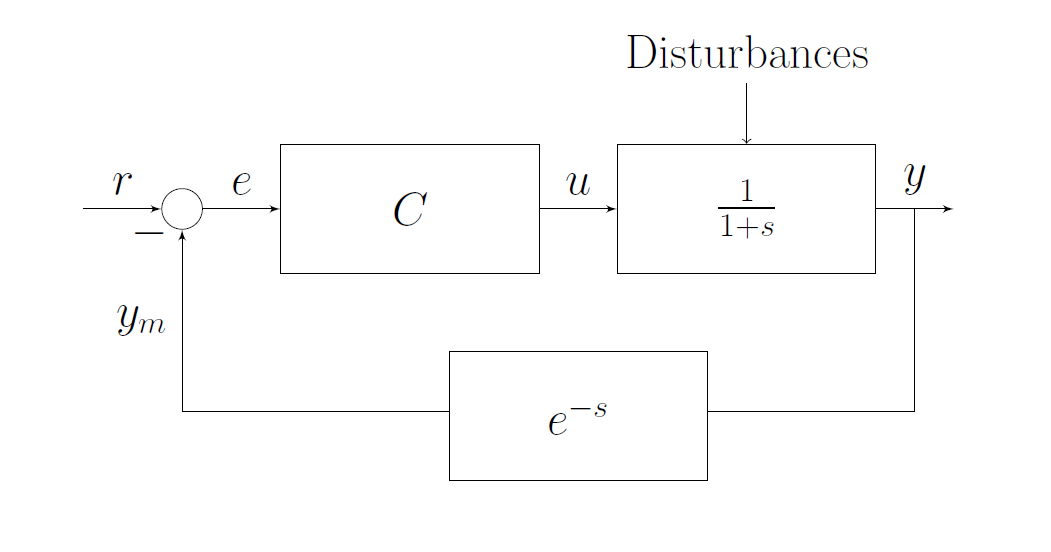
\includegraphics[width=250px]{graphics/lti-system}
	\caption{\acs{LTI} System}
	\label{fig:lti_system}
\end{figure}
\end{comment}

\par
To start, select the components that represent your system from the Simulink
Browser Library (see Figure \ref{fig:simulink_browser}). These could
include sources (e.g., steps), transfer blocks (e.g., functions) and sinks
(e.g., scopes) among many other types of building blocks.

\begin{figure}[h]
	\centering
	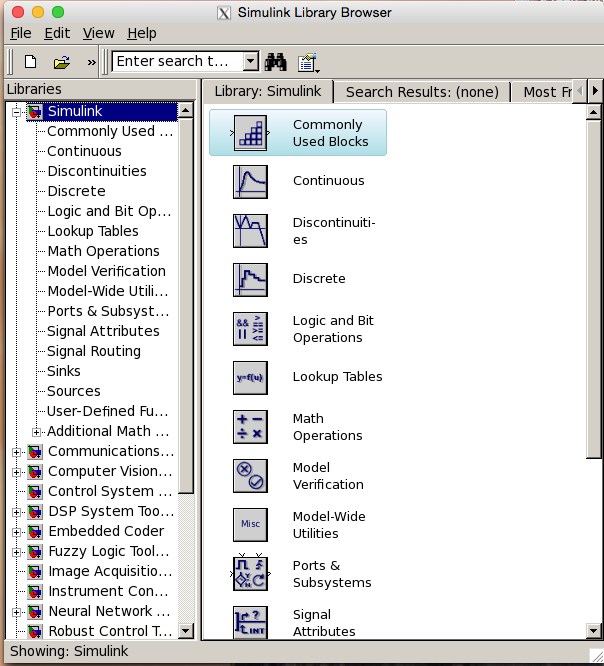
\includegraphics[width=200px]{graphics/simulink-browser}
	\caption{Simulink Library Browser}
	\label{fig:simulink_browser}
\end{figure}

\par
Provided that you have assembled your system correctly, you can simulate it
by clicking the {\texttt Simulation/\-Start} menu item. Figure
\ref{fig:simulink_lti} depicts the above \ac{LTI} system and simulation
result in Simulink using the Ziegler-Nichols method for the \ac{PID} controller
gains.

\begin{comment}
\begin{figure}[h]
	\centering
	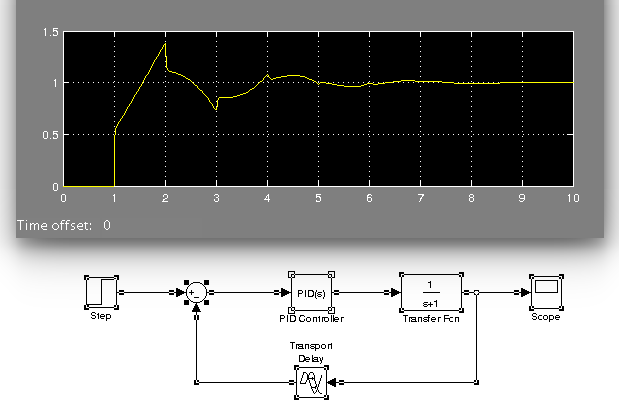
\includegraphics[width=250px]{graphics/simulink-lti}
	\caption{Simulink \acs{LTI} System}
	\label{fig:simulink_lti}
\end{figure}
\end{comment}

\begin{comment}
\par
Many complex systems are composed of similar basic components that possess
reoccurring transfer functions. Simulink provides an extensive library of these
building blocks and can be used if governing equations of complex systems shall
not be derived explicitly.
\newline
\end{comment}

\section{Group Members}
\label{sec:group_members}
csc$586$a-ernest-aaron-v$00815728$\\
csc$586$a-simar-arora-v$00824821$\\
csc$586$a-harshit-jain-v$00827753$\\
csc$586$a-stephan-heinemann-v$00814821$

\clearpage
\label{appendix}
\section{Acronyms}
\label{acronyms}

\begin{acronym}
	\acro{FIFO}{First-In First-Out}
		First-In First-Out is a method for organizing and manipulating a data buffer,
		where the oldest (first) entry, or 'head' of the queue, is processed first.
		\footnote{https://en.wikipedia.org/wiki/FIFO\_computing\_and\_electronics}
	\acro{LTI}{Linear Time-Invariant}
		Linear time-invariant theory comes from applied mathematics and has
		direct applications in NMR spectroscopy, seismology, circuits, signal
		processing, control theory, and other technical areas. It investigates
		the response of a linear and time-invariant system to an arbitrary
		input signal.
		\footnote{https://en.wikipedia.org/wiki/LTI\_system\_theory}
	\acro{MATLAB}{Matrix Laboratory}
		Matrix Laboratory is a multi-paradigm numerical computing environment
		and fourth-generation programming language.
		\footnote{https://en.wikipedia.org/wiki/MATLAB}
	\acro{PID}{Proportional Integral Derivative}
		A proportional-integral-derivative controller is a control loop
		feedback mechanism (controller) widely used in industrial control
		systems.
		\footnote{https://en.wikipedia.org/wiki/PID\_controller}
\end{acronym}

\clearpage
\label{bibliography}
\bibliographystyle{plain}
\bibliography{csc-586a-22}

\end{document}
